%%===============================================================================
% Document configuration

%%-------------------------------------------------------------------------------
% Document type
\documentclass[utf8]{FrontiersinHarvard}

%%-------------------------------------------------------------------------------
% Package configuration
\usepackage                                                                     % LaTeX Packages
{
    amsmath,                                                                    % Miscellaneous enhancements for mathematics
    amssymb,                                                                    % Math symbols
    booktabs,                                                                   % Extend tables
    tabularx,                                                                   % Add more contol to tables
    cite,                                                                       % Improved citation mechanims
    graphicx,                                                                   % Enhance graphics
    multirow,                                                                   % Create tables spanning multiple rows
    subcaption,                                                                 % Subcaptions in subfigures
    tikz,                                                                       % Generate figures in LaTeX
    xcolor,                                                                     % Colors
    microtype,
    lineno,                                                                     % Add line numbers to page
}

\linenumbers
\usetikzlibrary{automata, positioning, arrows.meta}                             % Tikz macros
\graphicspath{ {./img/} }                                                       % Paths to find images

%%-------------------------------------------------------------------------------
% Custom Commands
\newcommand{\TODO}[1]{{\color{green} To do: #1}}                                % For adding notes to paper
\def\keyFont{\fontsize{8}{11}\helveticabold }

%%-------------------------------------------------------------------------------
% Authors
\def\keyFont{\fontsize{8}{11}\helveticabold }
\def\firstAuthorLast{Brown {et~al.}} %use et al only if is more than 1 author
\def\Authors{Alexander Brown\,$^{1,*}$, Greg Droge\,$^{2}$}
% Affiliations should be keyed to the author's name with superscript numbers and be listed as follows: Laboratory, Institute, Department, Organization, City, State abbreviation (USA, Canada, Australia), and Country (without detailed address information such as city zip codes or street names).
% If one of the authors has a change of address, list the new address below the correspondence details using a superscript symbol and use the same symbol to indicate the author in the author list.
\def\Address{$^{1}$Department of Electrical and Computer Engineering, Logan, UT, USA \\
$^{2}$Department of Electrical and Computer Engineering, Logan, UT, USA}
% The Corresponding Author should be marked with an asterisk
% Provide the exact contact address (this time including street name and city zip code) and email of the corresponding author
\def\corrAuthor{Alexander Brown}
\def\corrEmail{A01704744@usu.edu}

\author[\firstAuthorLast ]{\Authors} %This field will be automatically populated
\address{} %This field will be automatically populated
\correspondance{} %This field will be automatically populated

%%===============================================================================
% Title, Authors, Abstract, Keywords
\begin{document}
\onecolumn
\firstpage{1}

%%-------------------------------------------------------------------------------
% Title
\title{A Position Allocation Approach to the Scheduling of Battery Electric Bus Charging}

%%---------------------------------------------------------------------------------
% Create title
\maketitle

%%---------------------------------------------------------------------------------
% Abstract
\begin{abstract}
\TODO{revisit}Dependable charging schedules for an increasing interest of battery electric bus (BEB) fleets is a critical component to
a successful adoption. In this paper, a BEB charging scheduling framework that considers spatiotemporal schedule
constraints, route schedules, fast and slow charging, and battery charging dynamics is modeled as a mixed integer linear
program (MILP). The MILP is modeled after the berth allocation problem (BAP) in a modified form known as the position
allocation problem (PAP). Linear battery dynamics are included to model the charging and discharging of buses while at
the station and during their routes, respectively. The optimization coordinates BEB charging to ensure each BEB has
sufficient charge while using slow chargers where possible for sake of battery health. The model validity is
demonstrated with a randomly generated set of routes for 40 buses and 220 visits to the charging station. The results
show that the slow chargers are more readily selected and the charging and spatiotemporal constraints are met while
considering the battery dynamics.

\tiny
 \keyFont{ \section{Keywords:} Berth Allocation Problem (BAP), Position Allocation Problem (PAP), Mixed Integer Linear Program (MILP), Battery Electric
Bus (BEB), Scheduling} %All article types: you may provide up to 8 keywords; at least 5 are mandatory.
\end{abstract}

%%===============================================================================
% Paper

%%-------------------------------------------------------------------------------
% Introduction
\section{Introduction}
\label{sec:introduction}
The public transportation system is crucial in any urban area; however, the increased awareness and concern of
environmental impacts of petroleum based public transportation has driven an effort to reduce the pollutant footprint
\citep{DeFilippo2014, Xylia2018, Guida2017, Li2016}. Particularly, the electrification of public bus transportation via
battery power, i.e., battery electric buses (BEBs), has received significant attention \citep{Li2016}. Although the
technology provides benefits beyond reduction in emissions, such as lower driving costs, lower maintenance costs, and
reduced vehicle noise, battery powered systems introduce new challenges such as larger upfront costs, and potentially
several hours long ``refueling'' periods \citep{Xylia2018, Li2016}. Furthermore, the problem is exacerbated by the
constraints of the transit schedule to which the fleet must adhere, the limited amount of chargers available, and
the adverse affects in the health of the battery due to fast charging \citep{Lutsey2019}. This paper presents a
continuous scheduling framework for a BEB fleet that shares limited fast and slow chargers. This framework takes into
consideration linear charging dynamics and a fixed bus schedule while meeting a certain battery charge threshold throughout the day.

Many recent efforts have been made simultaneously solve the problems of scheduling and charging fleets and determining
the infrastructure upon which they rely, e.g., \citep{Wei2018,
Sebastiani2016, Hoke2014, Wang2017}. The added complexity of considering both the BEB charge scheduling and the
infrastructure problems necessitates simplifications for sake of computation. First, only fast chargers are utilized in
planning \citep{Wei2018, Sebastiani2016, Wang2017, Zhou2020, Liu2020, Yang2018, Wang2017a, Qin2016}. Second, significant
simplifications to the charging models are made. Some approaches assume full charge \citep{Wei2018, Wang2017, Zhou2020,
Wang2017a}. Others have assumed that the charge received is proportional to the time spent on the charger
\citep{Liu2020, Yang2018}, which can be a valid assumption when the battery state-of-charge (SOC) is below 80\% charge
\citep{Liu2020}.

\TODO{Need a better literature review} A host of techniques have been used to generate the optimal charging
schedule. \citep{Sebastiani2016} uses simulation alongside an optimization strategy to identify charging station locations and
average stop times to supply enough charge for BEBs to complete their routes. \citep{Wei2018} utilizes a network flow
approach to optimize the deployment strategy of BEBs; however, the focus is primarily on replacing diesel or CNG buses.
In \citep{Hoke2014}, the focus is on developing a strategy to optimally charge batteries for electric vehicles
considering different sources of battery degradation. \citep{Wang2017} addresses a similar problem as this paper where the overall objective is to minimize the
annual total electric bus recharging system operating costs. Similarly to other works, such as \citep{Wei2018}, discrete
network flow approaches are utilized. Although effective, having to discretize the system introduces variables scaled
proportionally to the fidelity of the discretization of the model. This work attempts to remedy this by utilizing the
Position Allocation Problem (PAP) which utilizes a continuous model to describe the system.

This work builds upon the Position Allocation Problem, a modification of the Berth Allocation Problem (BAP), as a means to schedule the charging of electric vehicles \citep{Qarebagh2019}. The BAP solves the problem of allocating space
for incoming vessels to be berthed. Each arriving vessel requires both time and space to be serviced and is assigned a
berthing location \citep{Imai2001}. Vessels are lined up parallel to the berth to be serviced and are horizontally queued
as shown in Fig \ref{subfig:bapexample}. The PAP utilizes this notion of queuing for scheduling vehicles
to be charged, as shown in Fig \ref{subfig:papexample}. The PAP is formulated as a rectangle packing problem by assuming that vehicle charging will take a fixed amount of time, the amount of vehicles that can charge is limited by the physical width of the vehicles, and each vehicle visits the charger a single time \citep{Qarebagh2019}.

The main contribution of this work is the extension of the PAP to BEB charger scheduling. This includes modeling and
incorporation of a proportional charging model into the MILP framework, consideration of multiple charger types, and
inclusion of the route schedule for each bus. The result is a MILP formulation that coordinates charging times and
charger type for every visit that each bus makes to the station while considering a dynamic charge model and scheduling
constraints.

The remainder of the paper proceeds as follows: In Section \ref{sec:positionallocationproblem}, the PAP is introduced
with a formulation of the resulting MILP. Section \ref{sec:problemformulation} constructs the MILP for BEB scheduling, including modifications to the PAP queuing constraints and development of a dynamic charging model. Section \ref{sec:example} demonstrates an example of using the formulation to coordinate 40 buses over 220 total visits to the station. The paper ends in Section
\ref{sec:conclusion} with concluding remarks.

%%-------------------------------------------------------------------------------
% The Position Allocation Problem
\section{The Position Allocation Problem}
\label{sec:positionallocationproblem}
The BEB charge schedule formulation in this work builds upon the PA, which, in turn, builds upon the BAP. This section provides a brief overview of the BAP and a detailed formulation of PAP as
presented in \citep{Qarebagh2019}.

\subsection{Overview of BAP}
The BAP is a rectangle packing problem where a set
of rectangles ($\mathbb{O}$) are attempted to be optimally placed in a larger rectangle ($O$) as shown in Fig
\ref{fig:packexample}. The rectangle packing problem is an NP-hard problem that can be used to describe many real life
problems \citep{Bruin2013,Murata1995}. In some of these problems, the dimensions of $\mathbb{O}$ are held constant such
as in the problem of packing modules on a chip, where the widths and height of the rectangles represent the physical
width and heights of the modules \citep{Murata1995}. Other problems, such as the BAP, in some formulations, allow one side of
the rectangle to vary depending on its assigned position (i.e. the handling time is dependent on the berth)
\citep{Buhrkal2010}.

The BAP solves the problem of optimally assigning incoming vessels to berth positions to be serviced (Fig
\ref{subfig:bapexample}). The width and height of $O$ represent the berth length $S$ and time horizon $T$, respectively.
Similarly, the width and height for $\mathbb{O}$ represent the time spent to service vessel $i$ and the space taken by
docking vessel $i$, respectively. The vessel characteristics (length of the vessel, arrival time, handling time, desired
departure time) are assumed to be known for all $N$ vessels to be serviced. A representation of a BAP solution is shown
in Fig \ref{fig:bap}.

The BAP objective is generally represented as minimizing some operational time for a given vessel $i$. The operational
time may be chosen to minimize the difference between arrival and departure times, time spent being serviced, or overall
waiting time \citep{Voss2007, Buhrkal2010,Frojan2015}. The model must then constrain the vessel placement as to not allow
overlap spatially or temporally.

\subsection{The PAP Formulation}
The BAP formulation forms the basis of the PAP; however, there are some differences in the way the variables are
perceived. For the $i^{th}$ visit, starting service time, $u_i$, is now the starting charge time, the berth location,
$v_i$, is now the charger queue for assignment, and the service time, $p_i$, is now the time to charge. The PAP utilizes a number of parameters. The following parameters are constants.
\begin{itemize}
	\item $S$   : charger length
	\item $T$   : time horizon
	\item $N$   : number of incoming vehicles
	\item $p_i$ : charging time for vehicle $i;\; 1 \leq i \leq N$
	\item $s_i$ : width of vehicle $i;\; 1 \leq i \leq N$
	\item $a_i$ : arrival time of vehicle $i;\; 1 \leq i \leq N$
\end{itemize}
These constants define the problem bounds. The following list provides a series of decision variables used in the formulation.
\begin{itemize}
    \item $u_i$         : starting time of service for vehicle $i;\; 1 \leq i \leq N$
    \item $v_i$         : charge location $i;\; 1 \leq i \leq N$
    \item $c_i$         : departure time for vehicle $i;\; 1 \leq i \leq N$
    \item $\sigma_{ij}$ : binary variable that determines ordering of vehicles $i$ and $j$ in time
    \item $\delta_{ij}$ : binary variable that determines relative position of vehicles $i$ and $j$ when charging simultaneously
\end{itemize}
To determine the values for each of these decision variables, a MILP is formulated in \citep{Qarebagh2019} and shown here for sake of completeness.

begin{equation}
	\label{eq:bapobjective}
	\min\; \sum_{i=1}^N (c_i - a_i)
\end{equation}
Subject to:
\begin{subequations}
\label{eq:bapconstrs}
\begin{align}
    u_j - u_i - p_i - (\sigma_{ij} - 1)T \geq 0                   \label{subeq:baptime}         \\
    v_j - v_i - s_i - (\delta_{ij} - 1)S \geq 0                   \label{subeq:bapspace}        \\
    \sigma_{ij} + \sigma_{ji} + \delta_{ij} + \delta_{ji} \geq 1  \label{subeq:bapvalid_pos}    \\
    \sigma_{ij} + \sigma_{ji} \leq 1                              \label{subeq:bapsigma}        \\
    \delta_{ij} + \delta_{ji} \leq 1                              \label{subeq:bapdelta}        \\
    p_i + u_i = c_i                                               \label{subeq:bapdetach}       \\
    a_i \leq u_i \leq (T - p_i)                                   \label{subeq:bapvalid_starts} \\
    \sigma_{ij} \in \{0,1\},\;\delta_{ij} \in \{0,1\}\;           \label{subeq:bapsdspace}      \\
    v_i \in [0 \mbox{ } S ]                                       \label{subeq:bapvspace}
\end{align}
\end{subequations}

\noindent

The objective function \eqref{eq:bapobjective} minimizes the time spent to service each vehicle by minimizing over the
sum of differences between the departure time, $c_i$, and arrival time, $a_i$. i.e., It seeks to get each vehicle charged and on its way as quickly as possible.

Constraints \ref{subeq:baptime}-\ref{subeq:bapdelta} are used to ensure that individual rectangles do not overlap. For the PAP, they ensure that two vehicles charging simulateously are at different positions and, similarly, two vehicles that have overlapping positions do not overlap temporally. Constraint \eqref{subeq:baptime} establishes temporal ordering when active ($\sigma_{ij}=1$). Similarly, when $\delta_{ij} =1$ in \eqref{subeq:bapspace} then spatial ordering is established. Constraints \ref{subeq:bapvalid_pos}-\ref{subeq:bapdelta} enforce that spatial and/or temporal ordering is established between each possible vehicle pair. Constraints \eqref{subeq:bapsigma} and \eqref{subeq:bapdelta} enforce consistency. For example, \eqref{subeq:bapsigma} enforces that vehicle $i$ cannot come before vehicle $j$ and vehicle $j$ simultaneously come before vehicle $i$.

The last constraints force relationships between arrival time, charge start time, and departure time. Constraint
\eqref{subeq:bapdetach} states that the service start time, $u_i$, plus the time to service vehicle $i$, $p_i$, must
equal the departure time, $c_i$. Constraint \eqref{subeq:bapvalid_starts} enforces the arrival time, $a_i$, to be less
than or equal to the service start time, $u_i$, which in turn must be less than or equal to the latest time the vehicle
may begin to be serviced to stay within the time horizon. Constraint \eqref{subeq:bapsdspace} ensures that $\sigma_{ij}$ and
$\delta_{ij}$ are binary. Constraint \eqref{subeq:bapvspace} ensures that the assigned value of $v_i$ is a valid charging
position.

%%-------------------------------------------------------------------------------
%
\section{Problem Formulation}
\label{sec:problemformulation}
Applying the PAP to BEB charging requires four fundamental changes. The first is that the time that a BEB spends charging is allowed to vary. Thus, $p_i$ becomes a variable of optimization. Second, in the PAP each charging visit is assumed to be a different vehicle. For the BEB charging problem, each bus may make multiple visits to the station throughout the day and the resulting charge for a bus at a given time is dependent upon each of the prior visits made. Third, in the PAP, the charger is one continuous bar with vehicle width effectively restricting the number of vehicles charging simultaneously. For the BEB, it is assumed that a specific number of chargers exist and these chargers can charge the vehicle at a different rate. The fourth fundamental change is related to the first three. The charge of each bus must be tracked in the optimization to ensure that charging across multiple visits is sufficient to allow each bus to execute its route throughout the day.

% Variable table
\begin{table}[!htpb]
  \caption{Notation used throughout the paper}
  \label{tab:variables}
  \centering
  \begin{tabularx}{\textwidth}{l l}
    \toprule
    \textbf{Variable} & \textbf{Description}                                                                               \\
    \toprule
    \multicolumn{2}{l}{Input values}                                                                                       \\
    $n_B$        & Number of buses                                                                                         \\
    $M$          & An arbitrary very large upper bound value                                                               \\
    $n_V$        & Number of total visits                                                                                  \\
    $n_Q$        & Number of queues                                                                                        \\
    $n_C$ 	 & Number of chargers                                                                                      \\
    $\mathbb{V}$ & Set of visit indices, $\mathbb{V} = \{1, ..., n_V\}$                                                    \\
    $\mathbb{B}$ & Set of bus indices, $\mathbb{B} = \{1, ..., n_B\}$                                                      \\
    $\mathbb{Q}$          & Set of queue indices, $\mathbb{Q} = \{1, ..., n_Q\}$                                                             \\
    $i,j$        & Indices used to refer to visits                                                                         \\
    $b$ 	 & Index used to refer to a bus                                                                            \\
    $q$ 	 & Index used to refer to a queue                                                                          \\
    \toprule
    \multicolumn{2}{l}{Problem definition parameters}                                                                      \\
    $\Gamma$   & $\Gamma: \mathbb{V} \rightarrow \mathbb{B}$ with $\Gamma_i$ used to denote the bus for visit $i$                                   \\
    $\alpha_i$ & Initial charge percentage time for visit $i$                                                                   \\
    $\beta_i$ & Final charge percentage for bus $i$ at the end of the time horizon                                             \\
    $\epsilon_q$ & Cost of using charger $q$ per unit time                                                                        \\
    $\Upsilon$   & $\Upsilon: \mathbb{V} \rightarrow \mathbb{V}$ mapping a visit to the next visit by the same bus with $\Upsilon_i$ being the shorthand. \\
    $\kappa_b$ & Battery capacity for bus $b$                                                                                   \\
    $\lambda_i$ & Discharge of visit over route $i$                                                                              \\
    $\nu_b$ & Minimum charge percentage allowed for bus $b$                                                                  \\
    $\tau_i$ & Time visit $i$ must depart the station                                                                         \\
    $\zeta_b$ & Discharge rate for bus $b$                                                                                     \\
    $a_i$ & Arrival time of visit  $i$                                                                                     \\
    $i_0$ & Indices associated with the initial arrival for every bus in $A$                                               \\
    $i_f$ & Indices associated with the final arrival for every bus in $A$                                                 \\
    $m_q$ & Cost of a visit being assigned to charger $q$                                                                  \\
    $r_q$ & Charge rate of charger $q$ per unit time                                                                       \\
    \toprule
    \multicolumn{2}{l}{Decision Variables}                                                                                 \\
    $\delta_{ij}$ & Binary variable determining temporal ordering of vehicles $i$ and $j$                                       \\
    $\eta_i$    & Initial charge for visit $i$                                                                                \\
    $\sigma_{ij}$ & Binary variable determining the queue ordering between vehicles $i$ and $j$                                 \\
    $c_i$    & Ending charge time for visit $i$                                                                            \\
    $g_{iq}$ & The charge gain for visit $i$ from charger $q$                                                              \\
    $p_i$    & Amount of time spent on charger for visit $i$                                                               \\
    $u_i$    & Starting charge time of visit $i$                                                                           \\
    $v_i$    & Assigned queue for visit $i$                                                                                \\
    $w_{iq}$ & Binary assignment variable for visit $i$ to queue $q$                                                       \\
    \bottomrule
  \end{tabularx}
\end{table}


The discussion of the four changes are separated into two sections. Section \ref{sec:queuing} discusses the changes in the spatial-temporal constraint formulation to form a queuing constraint. Section \ref{sec:batt_dynamics} then discusses the addition of the bus charge management. This section ends with a brief discussion of a modified objective in Section \ref{sec:objective-function} and the statement of the full problem in Section \ref{sec:BEB_MILP}. The notation is explained throughout and summarized in Table \ref{tab:variables}.

\subsection{Queuing Constraints}
\label{sec:queuing}
\noindent
The queuing constraints help to ensure that the busses enter queues for charging or waiting as they come into the station. There are three sets to differentiate between different entities. $\mathbb{B} = \{1, ..., n_B\}$ is the set of bus indices with index $b$ used to denote an individual bus, $\mathbb{Q} = \{1, ..., n_Q\}$ is the set of queues with index $q$ used to denote an individual queue, and $\mathbb{V} = \{1, ..., n_V\}$ is a set of visits to the station with $i,j$ used to refer to individual visits. The mapping $\Gamma: \mathbb{V} \rightarrow \mathbb{B}$ is used to map a visit index to a bus index with the shorthand $\Gamma_i$ used to refer to the bus index for visit $i$.

Most variables are now defined in terms of a visit. Two separate visits could correspond to different buses or visits by the same bus. The spatial variable $s_i$ is removed and $v_i$ is made to be an integer corresponding to which queue visit $i$ will be using. Thus, when $\delta_{ij} = 1$, the visits must be at different chargers, i.e., $v_i-v_j \geq 1$. The variable $S$ is likewise replaced with $n_Q$. Note that $n_Q = n_B + n_C$, where $n_B$ is the number of busses and $n_C$ is the number of chargers. The rationale for having extra queues is to allow buses to sit idle instead of charging. The modified queuing constraints can be written as follows.
\begin{subequations}
\label{eq:packconstrs}
\begin{align}
    u_i - u_j - p_j - (\sigma_{ij} - 1)T \geq 0                      \label{subeq:time}         \\
    v_i - v_j - (\delta_{ij} - 1)n_Q \geq 1                            \label{subeq:space}        \\
    \sigma_{ij} + \sigma_{ji} + \delta_{ij} + \delta_{ji} \geq 1     \label{subeq:valid_pos}    \\
    \sigma_{ij} + \sigma_{ji} \leq 1                                 \label{subeq:sigma}        \\
    \delta_{ij} + \delta_{ji} \leq 1                                 \label{subeq:delta}        \\
    p_i + u_i = c_i                                                  \label{subeq:detach}       \\
    a_i \leq u_i \leq (T - p_i)                                      \label{subeq:valid_starts} \\
    c_i \leq \tau_i                                                  \label{subeq:valid_depart} \\
    p_i \geq 0                                                       \label{subeq:pos_charge} \\
    \sigma_{ij} \in \{0,1\},\;\delta_{ij} \in \{0,1\}                \label{subeq:sdspace}      \\
    v_i \in \mathbb{Q}                                           \label{subeq:vspace}
\end{align}
\end{subequations}

Constraints \eqref{subeq:time}-\eqref{subeq:valid_starts} and \eqref{subeq:sdspace} are nearly identical to those described in Section \ref{sec:positionallocationproblem} with the sole change in \eqref{subeq:space} being described above to conform to a queue.  Constraint \eqref{subeq:valid_depart} is added to ensure that the ending charge time, $c_i$, must be less than
or equal to the required departure time from the station, $\tau_i$. This enables the bus schedules to be considered during optimization. Finally, \eqref{subeq:vspace} enforces $v_i$ to be an integer in the set of possible queues.

\subsection{Battery Charge Dynamic Constraints}
\label{sec:batt_dynamics}
Using purely the constraints in \eqref{eq:packconstrs} with the objective in \eqref{eq:bapobjective} would result in
$c_i$ being chosen as small as possible by employing $p_i = 0,\; u_i = c_i$. Thus, the vehicles would not charge.
Furthermore, it does not encode any revisiting of the BEB to the charging station. To remedy this, battery dynamic
constraints are introduced.

Battery charge dynamic constraints are used to model the charge in each bus with the purpose of ensuring sufficient time is spent charging. Two constraints are enforced on the bus charge: busses must always have sufficient charge to execute their respective routes and each bus must end the day with a specific charge threshold, preparatory to execution for the next day.

The charge at the beginning of visit $i$ is denoted as $\eta_i$. As a charge on the bus is dependent upon the visits that bus makes to the station, the mapping $\Upsilon: \mathbb{V} \rightarrow \mathbb{V} \bigcup \{\varnothing\}$ is used to determine the next visit that corresponds to the same bus, with $\Upsilon_i$ being shorthand notation. Thus, $\Gamma_i$ and $\Gamma_{\Upsilon_i}$ would both map to the same bus index as long as $\Upsilon_i$ is not the null element, $\varnothing$. The null element is used to denote that there are no future visits by that same bus.

\TODO{Need to fix the following notation}
to drive time spent on the charger, $p_i$, as well as define initial, final,
and intermediate bus charges for each visit $i$. The initial and final bus charges are predefined and are represented by
the equations $\eta_{i_0} = \alpha_{i_0} \kappa_{i_0}$ and $\eta_{i_f} = \beta_{i_f} \kappa_{i_f}$, respectively, where $\alpha_{i_0}$ and $\beta_{i_f}$
are percentages of the battery capacity for the first and final visits for each bus, $b$, respectively. The intermediate
charges must be determined at solve time.

% To accomplish such a task, each arrival $i$ must be associated with an initial charge, $\eta_i$, which represents the
% charge received from the previous visit minus the discharge observed while on route. However, because the PAP assumes
% each arrival is unique, bus visits must be associated with a unique bus ID to appropriately initialize charges for each
% visit. This visit/ID pair is represented as vector denoted by $\Gamma$, where the index represents visit $i$ and the value is
% the bus ID. To propagate charges forward, another term $\Upsilon$ is introduced to represent the next index bus $i$ arrives.
% For example, assume $A = 3$ buses, $N = 5$ visits, and $\Gamma = [0,1,2,0,1]$. $\Gamma$ informs us that the first and fourth
% visits correspond to bus 1 and the second and fifth visits correspond to bus 2. As $\Upsilon$ maps from one visit to the next,
% it would take the value $\Upsilon = [3,4,-1,-1,-1]$, where 0-indexing is assumed and -1 represents no further visits for bus
% $\Gamma_i$.

It is assumed that the charge received is proportional to the time spent charging. The charge rate for charger $q$ is
denoted as $r_q$. Note that a value of $r_q = 0$ corresponds to a queue where no charging occurs. A bus in such a queue is simply waiting for the departure time. Thus, $n_Q = n_C + n_B$ where the final $n_B$ queues have $r_q = 0$ to allow an arbitrary number of buses to not charge at any given moment in time. The amount of discharge between visits $i$ and $\Upsilon_i$, the next visit of the same bus, is denoted as $\lambda_i$. If visit $i$ occurred at charger $q$, the charge of the bus coming into visit $\Upsilon_i$ would be
\begin{equation}
	\eta_{\Upsilon_i} = \eta_i + p_i r_q - \lambda_i.
\end{equation}

The binary decision variable $w_{iq}$ is introduced to determine whether visit $i$ uses charger $q$. This allows the
charge of the bus coming into visit $\Upsilon_i$ to be written in summation form as
\begin{subequations}
    \label{subeq:pre_next_charge}
\begin{align}
    \eta_{\Upsilon_i} = \eta_i + \sum_{q=1}^{n_Q} p_i w_{iq} r_q - \lambda_i  \\
    \sum_{q=1}^{n_Q} w_{iq} = 1 \\
    w_{iq} \in \{0,1\}
\end{align}
\end{subequations}
The choice of queue for visit $i$, $v_i$, becomes a slack variable and is defined in terms of $w_{iq}$ as
\begin{equation}
    v_i = \sum_{q=1}^{n_Q} qw_{iq}
\end{equation}

Maximum and minimum values for the charges are included to ensure the battery is not overcharged and to guarantee
sufficient charge for subsequent visits. The upper and lower battery charge bounds for bus $b$ are $\kappa_b$ and $\nu_b$, respectively. As $\eta_i$ corresponds to the charge at the beginning of the visit, the upper bound constraint must also include the charge received during the visit as follows.
\TODO{I changed the lower bound constraint as there is no real need to include the charge, but we may need to add in a final constraint.}
\begin{subequations}
    \label{subeq:pre_min_max}
\begin{align}
    \eta_i + \sum_{q=1}^{n_Q} p_i w_{iq} r_q \leq \kappa_{\Gamma_i}                 \\
    \eta_i + \geq \nu_{\Gamma_i}
\end{align}
\end{subequations}

Note that the term $p_i w_{iq}$ is a bilinear term (two decision variables being multiplied together) which is nonlinear
\citep{Rodriguez2013}. A standard way of linearizing a bilinear term that contains an integer variable is by introducing a slack variable with an either/or constraint \citep{Chen2010,Rodriguez2013}. Allowing
the slack variable $g_{iq}$ to be equal to $p_i w_{iq}$, $g_{iq}$ can be defined as
\begin{equation}
    \label{eq:giq_cases}
    g_{iq} =
    \begin{cases}
        p_i & w_{iq} = 1 \\
        0 & w_{iq} = 0
    \end{cases}.
\end{equation}
Equation \eqref{eq:giq_cases} can be expressed as a mixed integer constraint using big-M notation with the following four constraints. \TODO{Check to see if modification is correct}
\begin{subequations}
    \label{eq:slack_gain}
\begin{align}
    p_i - (1 - w_{iq})M \leq g_{iq}  \label{subeq:repgpgret} \\
    p_i \geq g_{iq}                 \label{subeq:repgples} \\
    Mw_{iq} \geq g_{iq}              \label{subeq:repgwgret} \\
    0 \leq g_{iq}                   \label{subeq:repgwles}
\end{align}
\end{subequations}

\noindent
where $M$ is a large value. If $w_{iq} = 1$ then \eqref{subeq:repgpgret} and \eqref{subeq:repgples} become $p_i \leq g_{iq}$ and $p_i \geq g_{iq}$, effectively stating $p_i = g_{iq}$ with \eqref{subeq:repgwgret} being inactive.
If $w_{iq} = 0$, \eqref{subeq:repgpgret} is inactive and \eqref{subeq:repgwgret} and \eqref{subeq:repgwles} force $g_{iq} = 0$.

\subsection{The BEB Charging Problem} \label{sec:BEB_MILP}
The goal of the MILP is to utilize chargers as little as possible to reduce energy costs with the fast charging penalized greater to reduce battery damage. \TODO{Can we just eliminate the $w_{iq} m_q$ term? }
Thus, an assignment cost $m_q$ and usage cost $\epsilon_q$ are associated with each charger, $q$. The cost for both the
assignment and utilization of slow chargers is less than that of the fast chargers. The objective function has an
assignment term, $w_{iq}m_q$, which is non-zero if charger $q$ is used for visit $i$. Similarly, a usage term $g_{iq}
\epsilon_q$ is non-zero only if charge is received for visit $i$ at charger $q$. The resulting objective is defined in Eq
\ref{eq:objective}. The assignment cost, $w_{iq}m_q$, and the usage cost, $g_{iq}\epsilon_q$, are summed over each visit, $i$,
and charger, $q$.
\begin{equation}
\label{eq:objective}
	\min \sum_{i=1}^N \sum_{q=1}^{n_Q} \Big( w_{iq} m_q + g_{iq} \epsilon_q \Big) \\
\end{equation}
Subject to the constraints in Eq \ref{eq:dynconstrs}.
\begin{multicols}{2}
\begin{subequations}
\label{eq:dynconstrs}
\begin{equation}
    u_i - u_j - p_j - (\sigma_{ij} - 1)T \geq 0                   \label{subeq:m_time}         \\
\end{equation}
\begin{equation}
    v_i - v_j - (\delta_{ij} - 1)n_Q \geq 1                       \label{subeq:m_space}        \\
\end{equation}
\begin{equation}
    \sigma_{ij} + \sigma_{ji} + \delta_{ij} + \delta_{ji} \geq 1                 \label{subeq:m_valid_pos}    \\
\end{equation}
\begin{equation}
    \sigma_{ij} + \sigma_{ji} \leq 1                                   \label{subeq:m_sigma}        \\
\end{equation}
\begin{equation}
    \delta_{ij} + \delta_{ji} \leq 1                                   \label{subeq:m_delta}        \\
\end{equation}
\begin{equation}
    p_i + u_i = c_i                                       \label{subeq:m_detach}       \\
\end{equation}
\begin{equation}
    a_i \leq u_i \leq (T - p_i)                                 \label{subeq:m_valid_starts} \\
\end{equation}
\begin{equation}
    c_i \leq \tau_i                                             \label{subeq:m_valid_depart} \\
\end{equation}
\begin{equation}
    \eta_{i_0} = \alpha_{i_0} \kappa_{\Gamma_{i_0}}                         \label{subeq:init_charge}    \\
\end{equation}
\begin{equation}
    \eta_i + \sum_{q=1}^{n_Q} g_{iq} r_q - \lambda_i = \eta_{\gamma_i}        \label{subeq:next_charge}    \\
\end{equation}
\begin{equation}
    \eta_i + \sum_{q=1}^{n_Q} g_{iq} r_q - \lambda_i \geq \nu_{\Gamma_i} \kappa_{\Gamma_i}      \label{subeq:min_charge} \\
\end{equation}
\begin{equation}
    \eta_i + \sum_{q=1}^{n_Q} g_{iq} r_q \leq \kappa_{\Gamma_i}              \label{subeq:max_charge}     \\
\end{equation}
\begin{equation}
    \eta_{i_f} \geq \beta_{i_f} \kappa_{\Gamma_{i_f}} \mbox{\TODO{confusing}} \label{subeq:final_charge}   \\
\end{equation}
\begin{equation}
    p_i - (1 - w_{iq})M \leq g_{iq}                          \label{subeq:gpgret}         \\
\end{equation}
\begin{equation}
    p_i \geq g_{iq}                                          \label{subeq:gples}          \\
\end{equation}
\begin{equation}
    Mw_{iq} \geq g_{iq}                                      \label{subeq:gwgret}         \\
\end{equation}
\begin{equation}
    0 \leq g_{iq}                                            \label{subeq:gwles}          \\
\end{equation}
\begin{equation}
    v_i = \sum_{q=1}^{n_Q} qw_{iq}                           \label{subeq:wmax}           \\
\end{equation}
\begin{equation}
    \sum_{q=1}^{n_Q} w_{iq} = 1                              \label{subeq:wone}           \\
\end{equation}
\begin{equation}
    w_{iq} \in \{0,1\}                                      \label{subeq:wspace}         \\
\end{equation}
\begin{equation}
    \sigma_{ij} \in \{0,1\},\;\delta_{ij} \in \{0,1\}\;                 \label{subeq:ssdspace}        \\
\end{equation}
\begin{equation}
    v_i \in  \mathbb{Q}                                              \label{subeq:vvspace}        \\
\end{equation}
\begin{equation}
    i \in \mathbb{V}                                        \label{subeq:vispace}         \\
\end{equation}
\begin{equation}
    q \in \mathbb{Q} 						  \label{subeq:qspace}
\end{equation}
\end{subequations}
\end{multicols}

Constraints \eqref{subeq:m_time}-\eqref{subeq:m_valid_depart} are reiterations of the queuing constraints in \eqref{eq:packconstrs}.
Constraints \eqref{subeq:init_charge}-\eqref{subeq:final_charge} provide initialization and terminal conditions as well
as intermediate constraints to provide continuity in vehicle charges. Constraint \eqref{subeq:init_charge} states the
first arrival for each bus is initialized with a charge of \TODO{fix:} $\alpha \kappa_{\Gamma_i}$.
Constraints \eqref{subeq:next_charge}, \eqref{subeq:min_charge}, and \eqref{subeq:max_charge} define the battery charge dynamics using \eqref{subeq:pre_next_charge} and \eqref{subeq:pre_min_max} with the gain slack variables $g_{iq}$ used in place of the bilinear term.
Constraints \eqref{subeq:gpgret} through \eqref{subeq:gwles} define $g_{iq}$ using \eqref{eq:slack_gain}.
% that the previous charge, $\eta_i$, plus the charging done by charger $q$ minus the discharge amount due to completing
% route, $\lambda_i$. This constraint is only used with indices with valid next visit values (i.e. $\Upsilon_i \neq -1$). Constraint
% \eqref{subeq:min_charge} is similar to \eqref{subeq:next_charge}, except it states that the initial charge, $\eta_i$, plus
% the charge from $q$ and the discharge from route, $\lambda_i$, must be greater than some percentage of its capacity,
% $\kappa_{\Gamma_i}$, in order to guarantee sufficient charge to complete the next route.
Constraint \eqref{subeq:max_charge} ensures that the charging done for visit $i$ cannot be greater than the capacity of the battery, $\kappa_{\Gamma_i}$. Constraint
\eqref{subeq:final_charge} states that the last visit for each vehicle must have a minimum charge of \TODO{update}$\beta \kappa_{\Gamma_i}$, guaranteeing a minimum initial charge for the next working day.
The last constraints \eqref{subeq:wspace}-\eqref{subeq:qspace} define the sets of valid values for each variable.

%================================================================================
% Example
\section{Example}
\label{sec:example}

An example will now be presented to demonstrate the utility of the developed MILP. A description of the scenario is
first presented followed by results.

\subsection{Scenario}
The given exampled utilizes $A = 40$ buses with $N = 220$ visits to the station divided between the $A$ buses. Each bus
has a 388 KWh battery that is required to stay above 25\% charge (97 KWh) to maintain battery health, and the bus is
assumed to begin the working day with 90\% charge (349 KWh). Additionally, each bus is required to end the day with a
minimum charge of 95\% (368 KWh). Planning is done over a 24-hour time horizon. $n_C = 9$ chargers are utilized where five
of the chargers are slow charging (100 KWh) and four are fast charging (400 KWh). As discussed in Section
\ref{sec:objective-function}, the slow chargers take longer, but are better for battery health than the fast chargers.
Therefore, the slow chargers are modeled with a lower cost than the fast chargers for both assignment, $m_q = r_q$, and
utilization, $\epsilon_q = r_q$, in the objective, \eqref{eq:objective}.

The bus schedules are randomly generated. It is assumed that each bus has no more than 30 minutes between route
departures. Bus routes are created by generating a random list of arrival times, assigning bus ID's to each visit, then
generating route durations. They may vary anywhere from a minimum of the average time between the current and next
arrival to a maximum of the next arrival time (i.e. $\frac{a_i + a_{\Upsilon_i}}{2}$ to $a_{\Upsilon_i}$). The discharge is assumed to
be linear and is calculated via $\lambda_i = \text{rand}(\frac{a_i + a_{\Upsilon_i}}{2},a_{\Upsilon_i})\zeta_{\Upsilon_i}$ where $1 \leq i \leq N$ and $\zeta_i$
is the discharge rate for each bus.

The optimization was performed using the Gurobi MILP solver \citep{Hespanha2018} on a machine running a quad-core Intel
i7-9700 4.7 GHz processor. The optimizer ran for 5 seconds to completion to produce the optimal solution.

\subsection{Results}
The schedule generated by the MILP is shown in Fig \ref{fig:schedule}. The top graph indicates the slow charger usage,
and the bottom indicates the fast charger usage. Although $9$ chargers were used, Fig \ref{fig:schedule} shows that
only five chargers were utilized.

Each color in Fig \ref{fig:schedule} is used to identify the bus ID assigned. It is noted that the overlaps in Fig
\ref{fig:schedule} indicate the waiting time of vehicle $j$ while vehicle $i$ charges. This is recognized by viewing the
vertical bars. These bars indicate the time bus $i$ is set to charge. The area before indicate waiting time and the area
after indicates the time spent on the charger. Note that, based upon vehicles needs, bus $i$ may arrive before bus $j$,
but wait until after bus $j$ charges before starting its charge (Fig \ref{fig:unoptimal}). This is an unintuitive
schedule caused by the cost of assignment parameter in the objective function, $m_q$. This type of constraint would not
be achieved through a greedy scheduling algorithm.

Fig \ref{fig:charges} depicts the charge for every bus over the time horizon. Every vehicle begins at 90\% charge,
finishes at 95\% charge, and never goes below 25\% in the intermediate arrivals as stated in the constraints
\eqref{eq:dynconstrs}. Fig \ref{fig:usage} represents the usage of each charger over the time horizon. The maximum
amount of slow chargers used at any given time is three and only one fast charger is utilized at a time.

The pattern, for the most part, in Fig \ref{fig:schedule} is to populate the first charger and supply the other chargers
as needed. Where this pattern primarily breaks down is around hour 15. Having moved each bus one charger down would have
resulted in the same cost. This behavior is due to a lack of cost for the amount of total chargers being utilized.
Adding a cost in the objective function to minimize the total amount of unique chargers would resolve this problem by
effectively attempting to ``pack'' the chargers down reducing the peak of Fig \ref{fig:usage}.

Although this formulation effectively discourages the use of fast chargers to utilize the more cost-effective slow
charges more readily, there is no consideration for the cost consumption and demand cost. Consumption cost accounts for
peak use of power in the system and demand cost accounts for the total energy used. These metrics are used to calculate
the monetary cost of the system. Calculating the demand cost would create more bilinear terms as the objective function
would have to sum over $\sum_{i=1}^N \sum_{q=1}^{n_Q} w_{iq}{r_q}(p_i)$, creating yet another linearization term. Furthermore, the
demand cost would require discretization of the system. The demand utilizes the peak energy consumption over 15 minute
intervals and uses the largest peak as the rate to charge. This would require tracking of when a charger is active and
including another variable to enable and disable $w_{iq}r_q$. This example displays the limitation of the MILP solver as
it adds effort and complexity to the system as a trade-off for calculating the optimal schedule. Other metaheuristic
solvers, such as simulated annealing (SA), would allow the problem to be solved without having to linearize the system.
\TODO{get the citation for this}

%%-------------------------------------------------------------------------------
% Conclusion
\section{Conclusion}
\label{sec:conclusion}
This work developed a MILP scheduling framework that optimally assigns slow and fast chargers to a BEB bus fleet
assuming a constant schedule. The BAP was introduced with an example formulation and was then compared to the PAP. The
PAP constructed on the BAP to allow the time spent on the charger, $p_i$, to be a decision variable. Because the
original PAP required service time, $p_i$, to be given, linear battery dynamics were introduced to drive charging times.
Additional constraints were also introduced to provide limits for the battery dynamics.

An example was presented that demonstrated the ability of the formulation to optimally select slow and fast chargers to
meet the requirements of the time schedule and the charge consumed during the bus routes. It was also observed that the
formulation was able to successfully create a charging schedule without creating conflicts (Fig \ref{fig:schedule}). The
charge for each bus was tracked in Fig \ref{fig:charges} and shows that the schedule maintained the charges between the
maximum charge, 100\%, and the minimum charge, 25\%.

Limitations were demonstrated in the lack of objective to limit the total amount of chargers utilized and to calculate
the demand and consumption costs. Further fields of interest are to utilize the formulation (Eq \eqref{eq:objective} and
\eqref{eq:dynconstrs}) with nonlinear battery dynamics, calculation and utilization of the demand and consumption cost
in the objective function, and utilizing this formulation in a metaheuristic solver.

%%================================================================================
% Bibliography
%\bibliographystyle{Frontiers-Harvard}
\bibliographystyle{plain}
\bibliography{main}

%%================================================================================
% Figures
\section*{Figure Captions}
%%--------------------------------------------------------------------------------
% BAP and PAP comparison
\begin{figure}
	\label{fig:bappap}
	\caption{Comparison between BAP and PAP}
	\centering
	\begin{subfigure}[b]{0.45\textwidth}
		\centerline{
		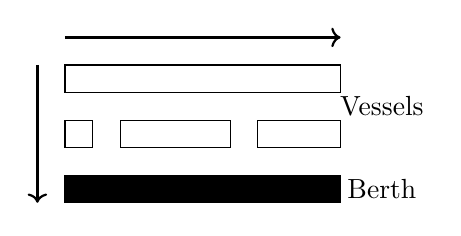
\begin{tikzpicture}[scale=0.35]
			\draw[rotate=90,fill=black] (0,0) rectangle (1,10);
			\draw[rotate=90](2,0) rectangle (3,3);
			\draw[rotate=90](2,4) rectangle (3,8);
			\draw[rotate=90](2,9) rectangle (3,10);
			\draw[rotate=90](4,0) rectangle (5,10);

			\draw[thick,->] (-11,5)--(-11,0);
			\draw[thick,->] (-10,6)--(0,6);

			\node at (1.5,0.5) {Berth};
			\node at (1.5,3.5) {Vessels};
		\end{tikzpicture}}
	\caption{Example of berth allocation. Vessels are docked in berth locations (horizontal) and are queued over time (vertical). The vertical arrow represents the movement direction of queued vessels and the horizontal arrow represents the direction of departure.}
		\label{subfig:bapexample}
	\end{subfigure}

	\begin{subfigure}[b]{0.45\textwidth}
		\centerline{
		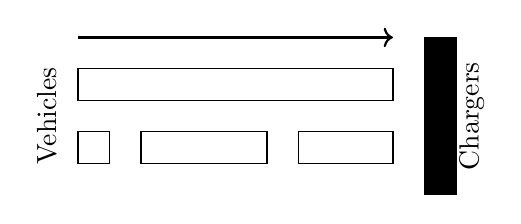
\begin{tikzpicture}[scale=0.4]
			\draw[fill=black] (0,0) rectangle (1,5);

			\draw[rotate=90](1,1) rectangle (2,4);
			\draw[rotate=90](1,5) rectangle (2,9);
			\draw[rotate=90](1,10) rectangle (2,11);
			\draw[rotate=90](3,1) rectangle (4,11);

			\draw[thick,->] (-11,5)--(-1,5);

			\node[rotate=90] at (-12,2.5) {Vehicles};
			\node[rotate=90] at (1.5,2.5) {Chargers};
		\end{tikzpicture}}
	\caption{Example of position allocation. Vehicles are placed in queues to be charged and move in the direction indicated by the arrow.}
		\label{subfig:papexample}
	\end{subfigure}
\end{figure}

%%--------------------------------------------------------------------------------
% Variable table
\begin{table}[!htpb]
  \caption{Notation used throughout the paper}
  \label{tab:variables}
  \centering
  \begin{tabularx}{\textwidth}{l l}
    \toprule
    \textbf{Variable} & \textbf{Description}                                                                               \\
    \toprule
    \multicolumn{2}{l}{Input values}                                                                                       \\
    $n_B$        & Number of buses                                                                                         \\
    $M$          & An arbitrary very large upper bound value                                                               \\
    $n_V$        & Number of total visits                                                                                  \\
    $n_Q$        & Number of queues                                                                                        \\
    $n_C$ 	 & Number of chargers                                                                                      \\
    $\mathbb{V}$ & Set of visit indices, $\mathbb{V} = \{1, ..., n_V\}$                                                    \\
    $\mathbb{B}$ & Set of bus indices, $\mathbb{B} = \{1, ..., n_B\}$                                                      \\
    $\mathbb{Q}$          & Set of queue indices, $\mathbb{Q} = \{1, ..., n_Q\}$                                                             \\
    $i,j$        & Indices used to refer to visits                                                                         \\
    $b$ 	 & Index used to refer to a bus                                                                            \\
    $q$ 	 & Index used to refer to a queue                                                                          \\
    \toprule
    \multicolumn{2}{l}{Problem definition parameters}                                                                      \\
    $\Gamma$   & $\Gamma: \mathbb{V} \rightarrow \mathbb{B}$ with $\Gamma_i$ used to denote the bus for visit $i$                                   \\
    $\alpha_i$ & Initial charge percentage time for visit $i$                                                                   \\
    $\beta_i$ & Final charge percentage for bus $i$ at the end of the time horizon                                             \\
    $\epsilon_q$ & Cost of using charger $q$ per unit time                                                                        \\
    $\Upsilon$   & $\Upsilon: \mathbb{V} \rightarrow \mathbb{V}$ mapping a visit to the next visit by the same bus with $\Upsilon_i$ being the shorthand. \\
    $\kappa_b$ & Battery capacity for bus $b$                                                                                   \\
    $\lambda_i$ & Discharge of visit over route $i$                                                                              \\
    $\nu_b$ & Minimum charge percentage allowed for bus $b$                                                                  \\
    $\tau_i$ & Time visit $i$ must depart the station                                                                         \\
    $\zeta_b$ & Discharge rate for bus $b$                                                                                     \\
    $a_i$ & Arrival time of visit  $i$                                                                                     \\
    $i_0$ & Indices associated with the initial arrival for every bus in $A$                                               \\
    $i_f$ & Indices associated with the final arrival for every bus in $A$                                                 \\
    $m_q$ & Cost of a visit being assigned to charger $q$                                                                  \\
    $r_q$ & Charge rate of charger $q$ per unit time                                                                       \\
    \toprule
    \multicolumn{2}{l}{Decision Variables}                                                                                 \\
    $\delta_{ij}$ & Binary variable determining temporal ordering of vehicles $i$ and $j$                                       \\
    $\eta_i$    & Initial charge for visit $i$                                                                                \\
    $\sigma_{ij}$ & Binary variable determining the queue ordering between vehicles $i$ and $j$                                 \\
    $c_i$    & Ending charge time for visit $i$                                                                            \\
    $g_{iq}$ & The charge gain for visit $i$ from charger $q$                                                              \\
    $p_i$    & Amount of time spent on charger for visit $i$                                                               \\
    $u_i$    & Starting charge time of visit $i$                                                                           \\
    $v_i$    & Assigned queue for visit $i$                                                                                \\
    $w_{iq}$ & Binary assignment variable for visit $i$ to queue $q$                                                       \\
    \bottomrule
  \end{tabularx}
\end{table}


%%--------------------------------------------------------------------------------
%
\begin{figure}[htbp]
	\centerline{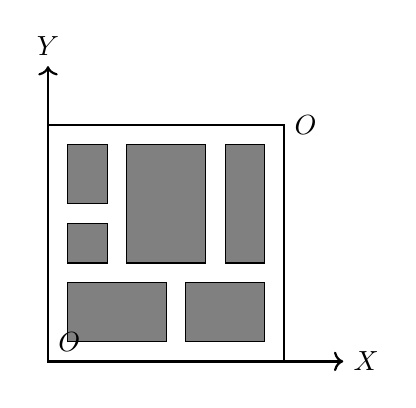
\begin{tikzpicture}[scale=0.25]
	    \draw [thick, -] (0,0) rectangle (12,12) node[right]{$O$};
	    \draw[fill=gray] (1,1) rectangle (6,4);
	    \draw[fill=gray] (11,11) rectangle (9,5);
	    \draw[fill=gray] (8,11) rectangle (4,5);
	    \draw[fill=gray] (1,11) rectangle (3,8);
	    \draw[fill=gray] (1,7) rectangle (3,5);
	    \draw[fill=gray] (11,1) rectangle (7,4);
        \draw [thick,<->] (0,15) node[above]{$Y$}                      --
                                 (0,0)node[above right]{$\mathbb{O}$} --
                                 (15,0) node[right]{$X$};
	\end{tikzpicture}}
	\caption{Example of rectangle packing problem}
	\label{fig:packexample}
\end{figure}

%%--------------------------------------------------------------------------------
% Spatial temporal graph representation
\begin{figure}[ht]
	\centerline{
	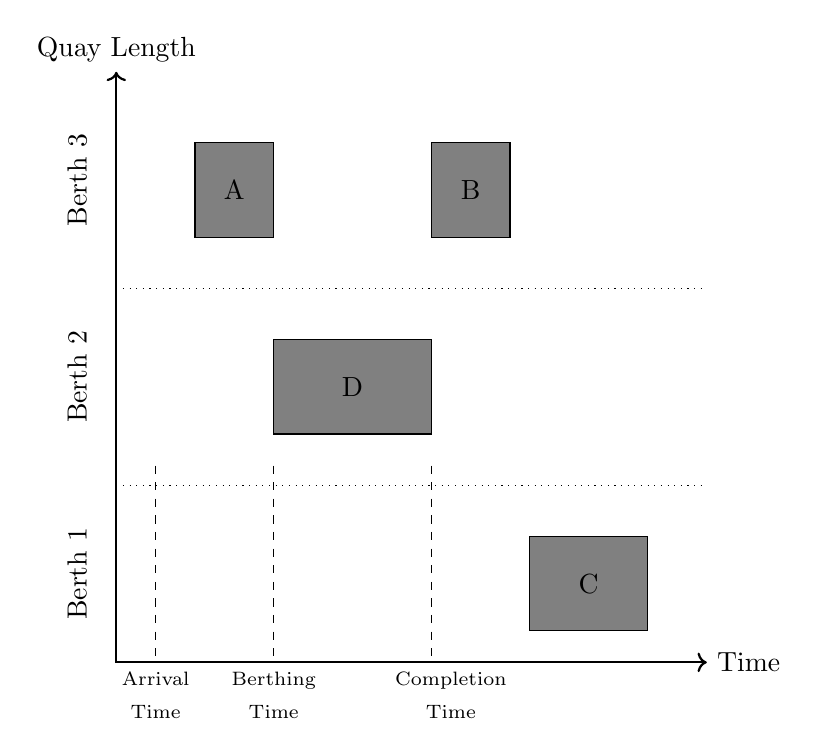
\begin{tikzpicture}[scale=0.5]
        \draw [thick,<->] (0,15) node[above]{Quay Length} --
                                 (0,0)                    --
                                 (15,0) node[right]{Time};
        \node[rectangle, draw, fill=gray, minimum width=1cm, minimum height = 1.2cm] at (3,12) {A};
        \node[rectangle, draw, fill=gray, minimum width=1cm, minimum height = 1.2cm] at (9,12) {B};
        \node[rectangle, draw, fill=gray, minimum width=2cm, minimum height = 1.2cm] at (6,7) {D};
        \node[rectangle, draw, fill=gray, minimum width=1.5cm, minimum height = 1.2cm] at (12,2) {C};

	\node [below,align=center] at (1.0,0) {\scriptsize Arrival\\ \scriptsize Time};
	\draw[dashed] (1.0,5)--(1.0,0);

	\node [below, align=center] at (4,0) {\scriptsize Berthing\\ \scriptsize Time};
	\draw[dashed] (4,5)--(4,0);

	\node [below, align=center] at (8.5,0) {\scriptsize Completion\\ \scriptsize Time};
	\draw[dashed] (8,5)--(8,0);

        \draw[dotted] (0, 4.5) -- (15, 4.5);
        \draw[dotted] (0, 9.5) -- (15, 9.5);

	\node[rotate=90] at (-1, 2.25) {Berth 1};
	\node[rotate=90] at (-1, 7.25) {Berth 2};
	\node[rotate=90] at (-1, 12.25) {Berth 3};

	\end{tikzpicture}
    }
	\caption{The representation of the berth-time space}
	\label{fig:bap}
\end{figure}

%%--------------------------------------------------------------------------------
%
\begin{figure}[htbp]
	\centerline{
	\begin{tikzpicture}[scale=0.35]
		\draw [thick,<->] (0,15) node[above]{Quay Length} --
					 (0,0)                                   --
					 (15,0) node[right]{Time};

		\node[rectangle, draw, minimum width=1.5cm, minimum height = 2cm] at (5,8) {$i$};
		\node[rectangle, draw, minimum width=1cm, minimum height = 1cm] at (2,2) {$j$};
		\node[rectangle, draw, dashed, minimum width=1cm, minimum height = 1.2cm] at (5,12) {$k_1$};
		\node[rectangle, draw, dashed, minimum width=1cm, minimum height = 1.2cm] at (7,6) {$k_3$};
		\node[rectangle, draw, dashed, minimum width=1cm, minimum height = 1.2cm] at (4,2) {$k_2$};
	\end{tikzpicture}
	}
	\caption{Examples of different methods of overlapping. Space overlap: $v_{k_1} < v_{i} + s_i \therefore \delta_{k_{1}i} = 0$. Time overlap $u_{k_1} < u_{j} + p_j \therefore \sigma_{k_{2}j} = 0$. Both space and time overlap $\sigma_{k_{3}i} = 0$ and $\delta_{k_{3}j} = 0$.}
	\label{fig:multipleassign}
\end{figure}

%%--------------------------------------------------------------------------------
%
\begin{figure}[htbp]
	\centering
	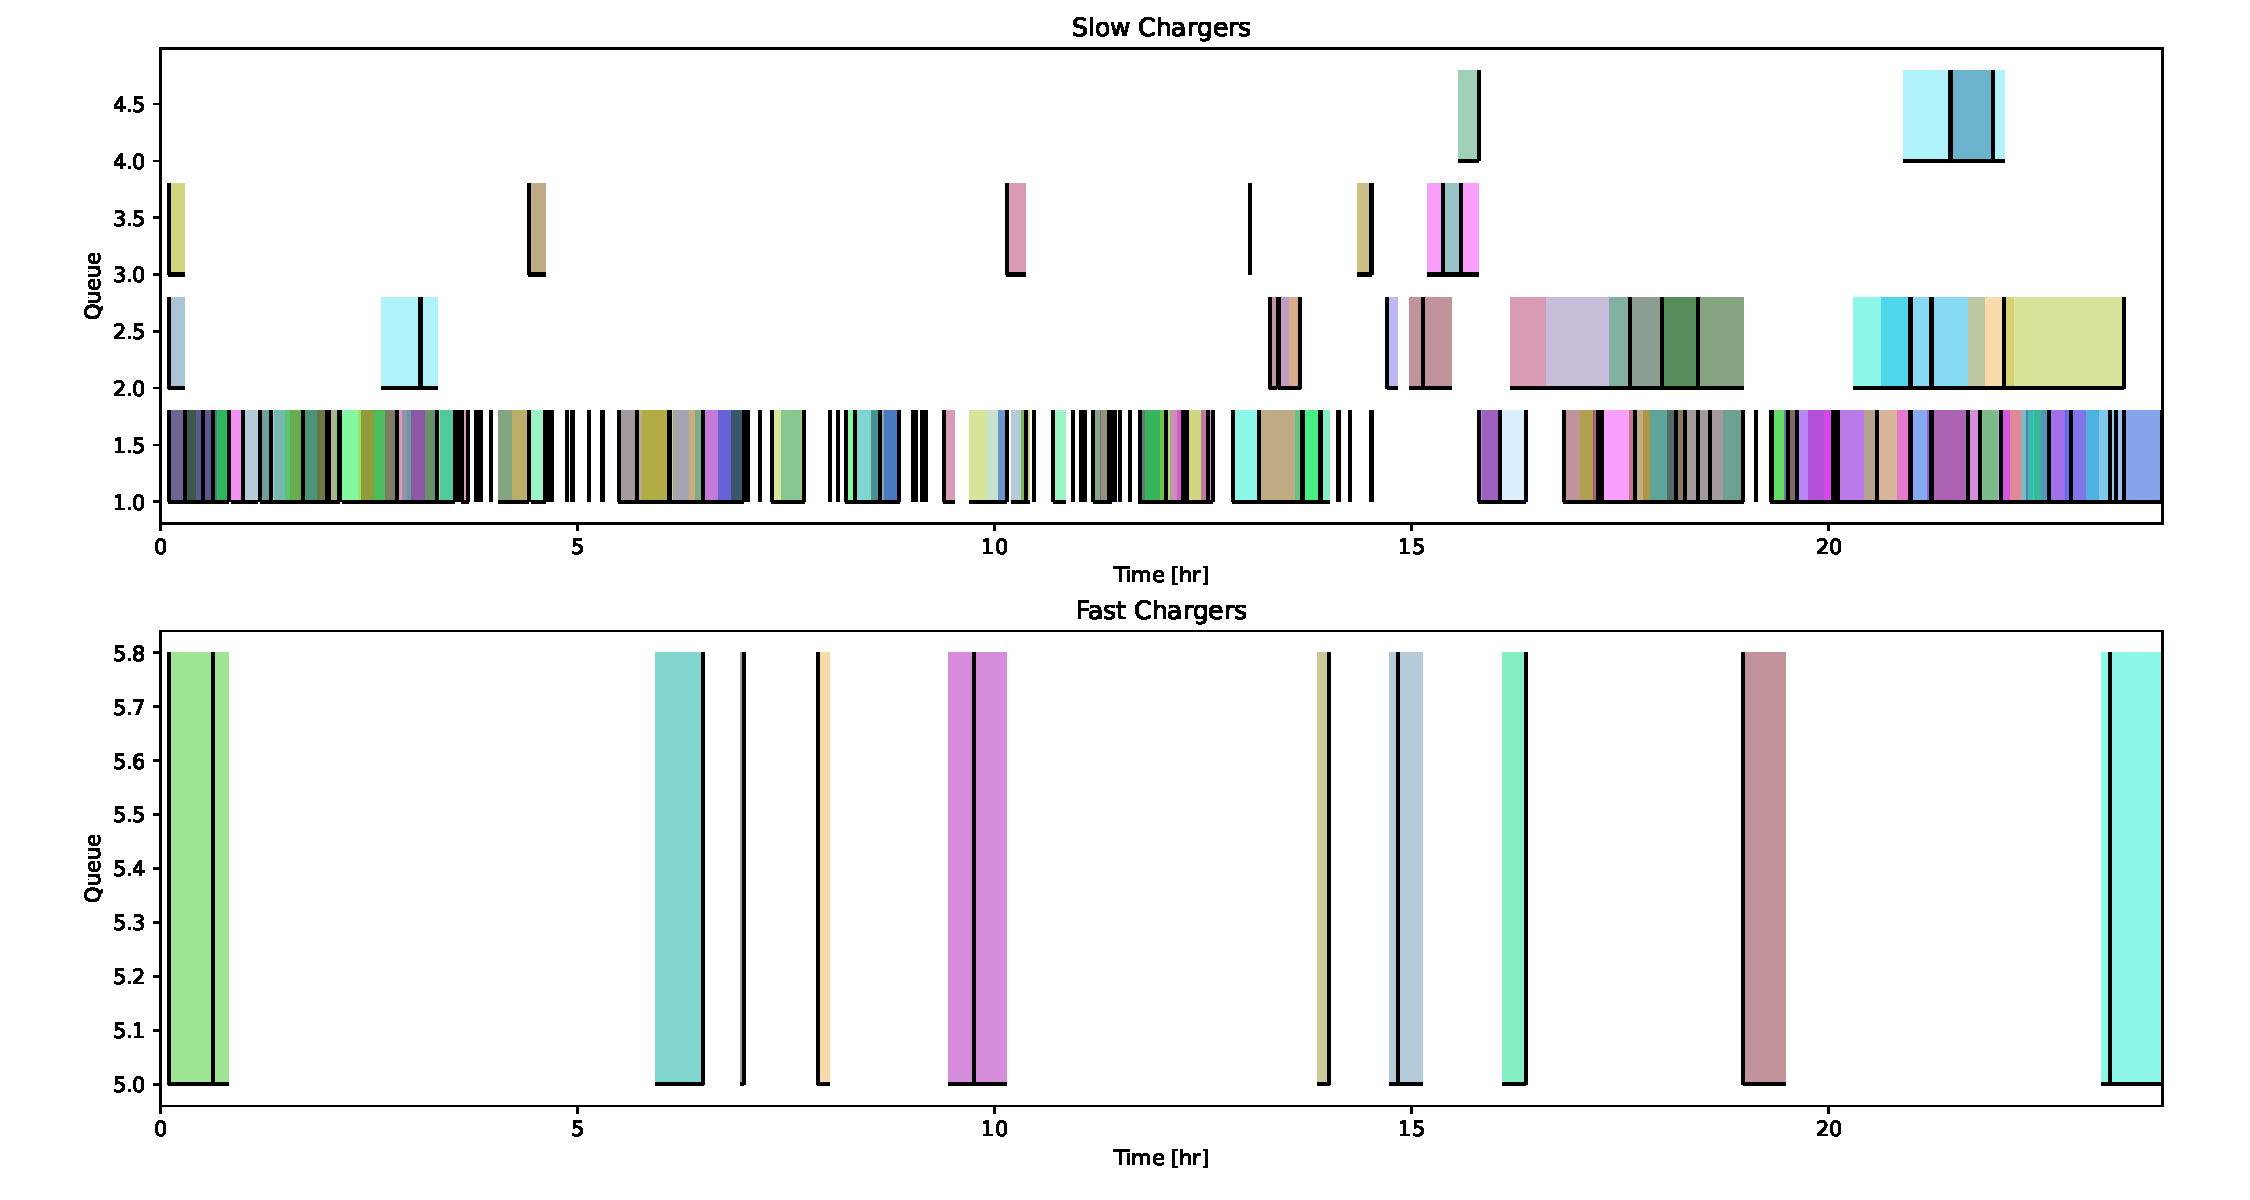
\includegraphics[trim=1in 0.25in 1in 0.5in, width=\linewidth]{schedule.pdf}
	\caption{Bus schedule generated with PAP MILP. Each color is assigned to a specific bus ID. The vertical bars indicate the time the vehicles are set to charge, the area before said bars indicate the waiting times for each visit $1 \leq i \leq N$. Similarly, the area after the bars indicate the time spent on the charger.}
	\label{fig:schedule}
\end{figure}

%%--------------------------------------------------------------------------------
%
\begin{figure}[htbp]
	\centering
	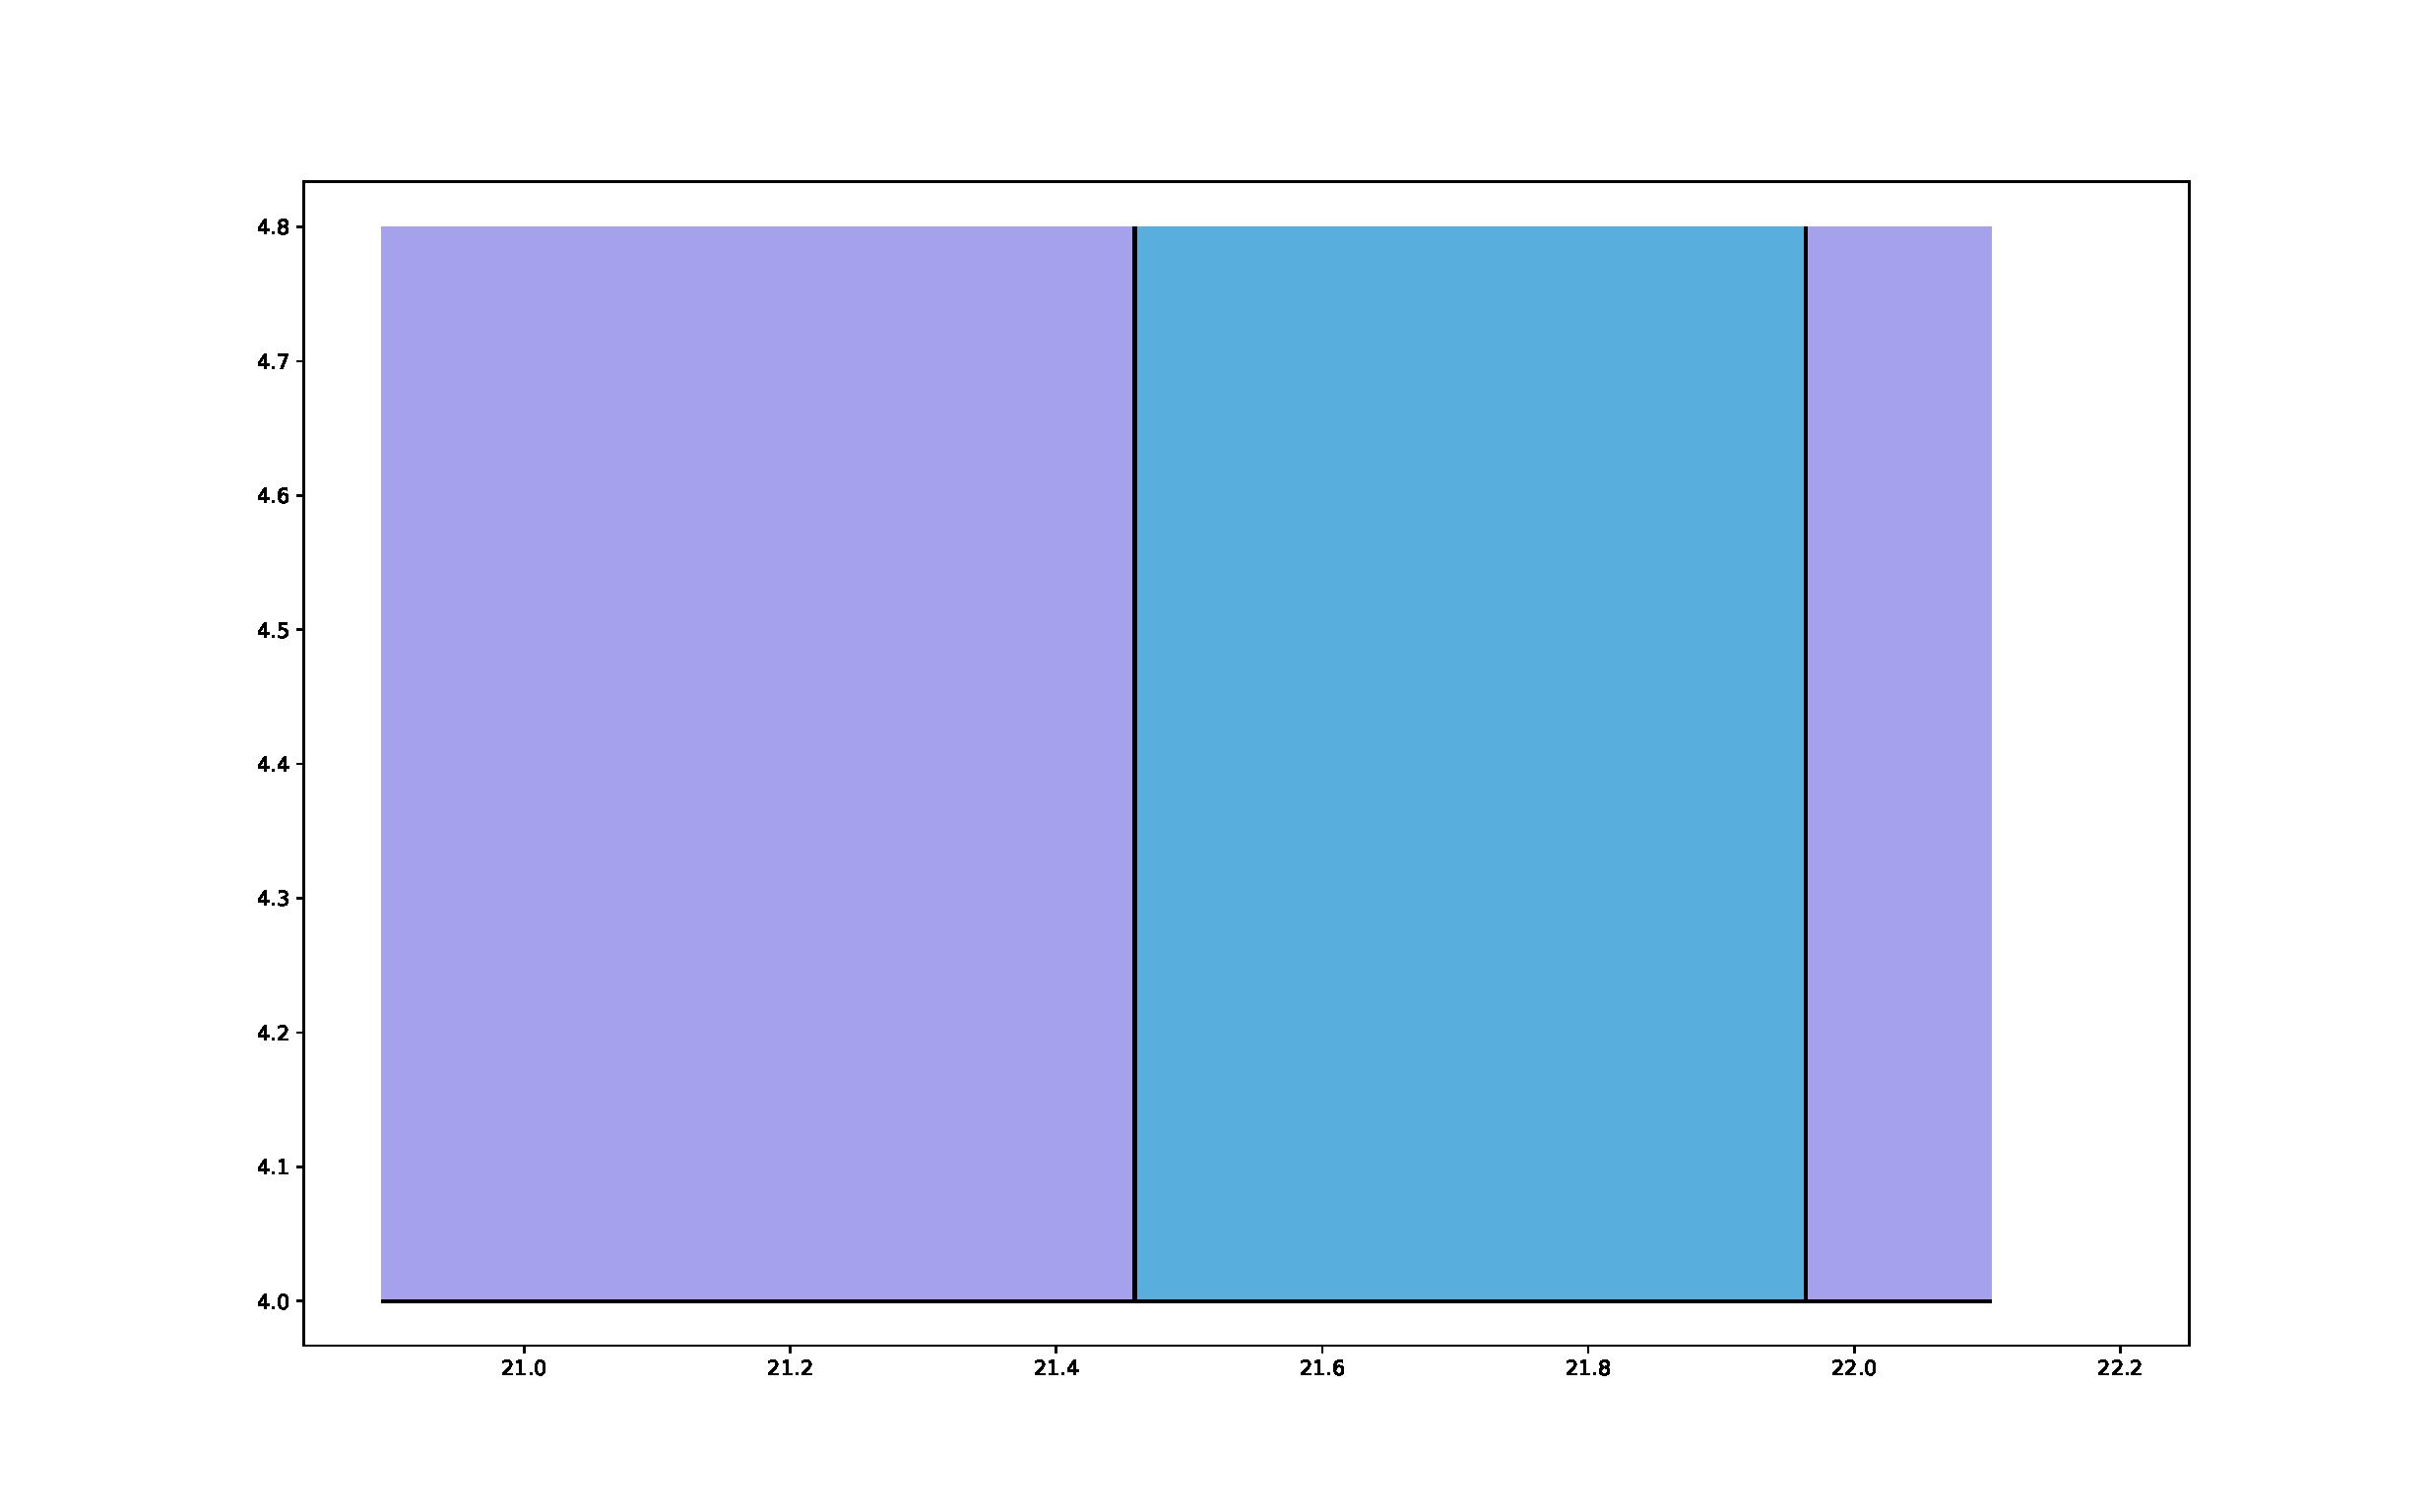
\includegraphics[trim=0in 0in 0in 0in, width=\linewidth]{unoptimal.pdf}
	\caption{An example, from Fig \ref{fig:schedule}, of a bus $i$ arriving before $j$, having $i$ wait for $j$ to arrive, and charge $i$ after $j$ is detached.}
	\label{fig:unoptimal}
\end{figure}

%%--------------------------------------------------------------------------------
%
\begin{figure}[htbp]
	\centering
	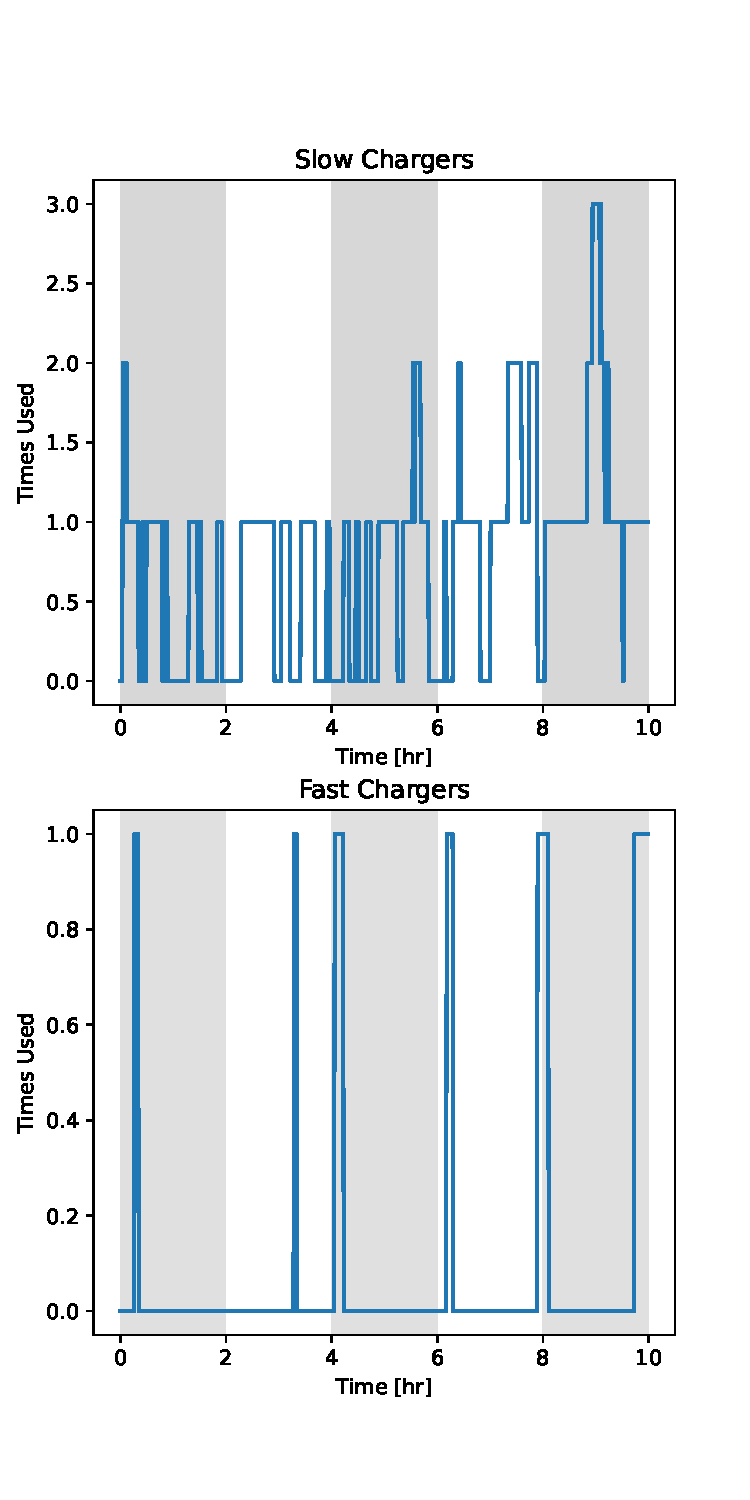
\includegraphics[trim=0in 0.25in 0in 0.75in, width=\linewidth]{usage.pdf}
	\caption{Amount of slow and fast chargers used at any given time.}
	\label{fig:usage}
\end{figure}

%%--------------------------------------------------------------------------------
%
\begin{figure}[htbp]
	\centering
	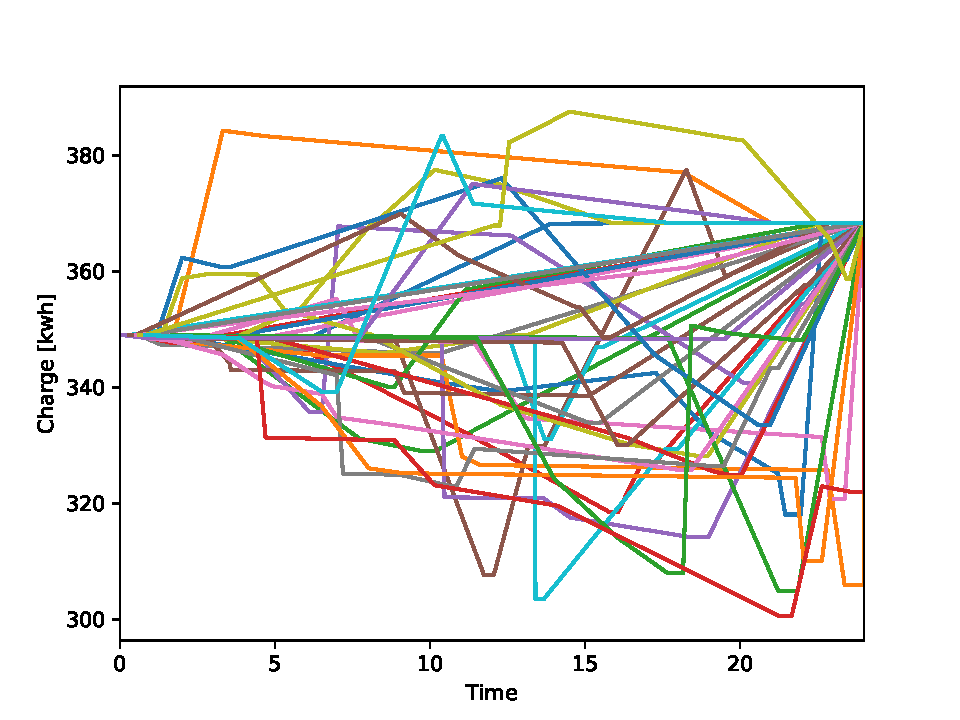
\includegraphics[trim= 0.25in 0in 0.5in 0.25in, width=\linewidth]{charges.pdf}
	\caption{Charge for each bus over the time horizon.}
	\label{fig:charges}
\end{figure}

%%%%%%%%%%%%%%%%%%%%%%%%%%%%%%%%%%%%%%%%%%%%%%%%%%%%%%%%%%%%%%%%%%%%%%%%%%%%%%%%%
\end{document}